\documentclass[11pt,a4paper]{scrartcl}
\usepackage[top=3cm,left=3cm,right=3cm,bottom=3cm]{geometry}
\usepackage[utf8]{inputenc}
\usepackage[pdftex]{hyperref}
\usepackage[T1]{fontenc}
\usepackage[ngerman]{babel}
\usepackage{graphicx}


\begin{document}

\section{Zielsetzung}
\begin{tabular}{|l|l|}
    \hline
    \textbf{Beschreibung} & \textbf{Typ} \\
    \hline
    Berechnung der Sitzverteilung im Bundestag & Muss \\
    \hline
    Batch-Loading von Stimmen & Muss \\
    \hline
    Wahlkreisübersicht & Muss \\
    \hline
    Anonymisierung der Stimmen & Muss \\
    \hline
    Stimmverteilung nach Bundesländern, Wahlkreisen, Parteien & Soll \\
    \hline
    Liste von Überhangmandaten & Soll \\
    \hline
    Kandidatenübersicht, Länderübersicht & Kann \\
    \hline
    Abgabe von Stimmen über API & Soll \\
    \hline
    Web-Frontend für Auswertung & Muss \\
    \hline
    Smartphone-App für Auswertung & Kann \\
    \hline
    Übersichtliche Quellcodeformatierung und -dokumentation & Muss \\
    \hline
\end{tabular}\\
\\
\\
Funktionen, die nicht implementiert werden sollen:
\begin{itemize}
    \item Benutzeroberläche zur Stimmeingabe
    \item Sicherstellung von einmaliger Stimmabgabe pro Person
\end{itemize}

\section{Technische Umsetzung}
\begin{itemize}
    \item Web-Frontend zum Anzeigen der Auswertung und Statistiken
    \item Hilfsanwendung zum Ändern der in der Datenbank gespeicherten Stimmen
    \item Bibliothek zum Zugriff auf Datenbank und für die Auswertung der Wahl
    \item Datenbank zur Speicherung der Stimm-Informationen
\end{itemize}
Interaktion zwischen den Modulen:\\
Das Web-Frontend verwendet die Bibliothek, um die vom Benutzer angeforderten
Auswertungen anzuzeigen, diese werden auf Basis der Datenbank generiert. Um
Stimmen in die Datenbank einzufügen gibt es eine Hilfsanwendung, die nicht
öffentlich zugänglich sein soll.



\newpage
\section{GUI-Entwürfe}
\begin{figure}[h!]
    \begin{center}
        \fbox{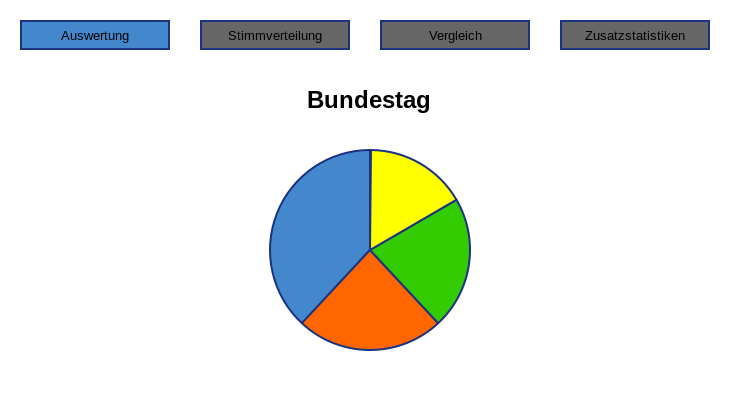
\includegraphics[width=1\textwidth]{01-Auswertung}}
    \end{center}
    \caption{Auswertung der Wahl - Bundestagszusammensetzung}
    \label{fig:gui-auswertung}
\end{figure}
$ $\newline
\begin{figure}[h!]
    \begin{center}
        \fbox{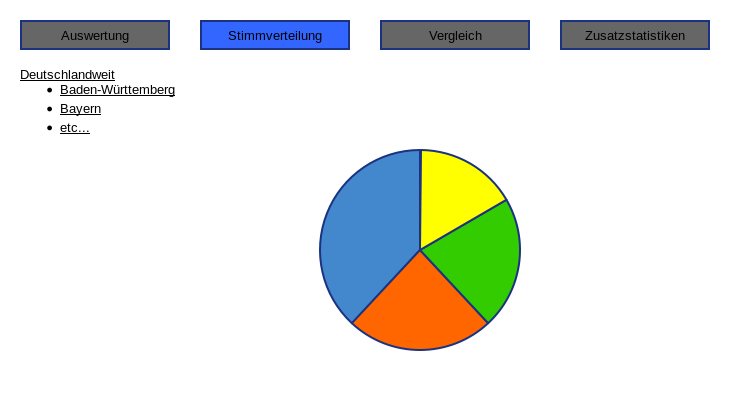
\includegraphics[width=1\textwidth]{02-Stimmverteilung}}
    \end{center}
    \caption{Stimmverteilung bundesweit, in Ländern und Wahlkreisen}
    \label{fig:gui-stimmverteilung}
\end{figure}
\begin{figure}[h!]
    \begin{center}
        \fbox{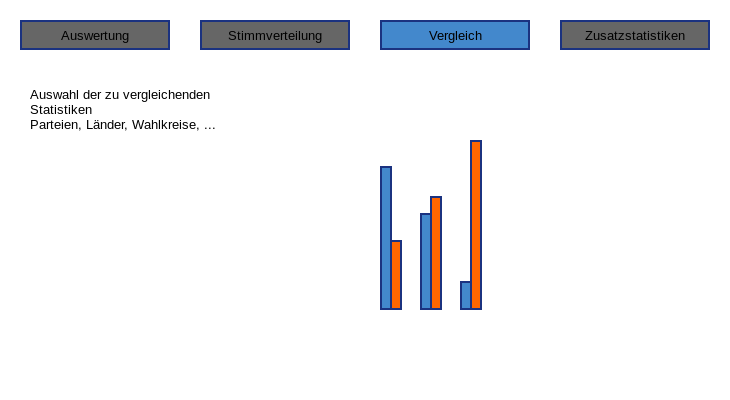
\includegraphics[width=\textwidth]{03-Vergleich}}
    \end{center}
    \caption{Vergleich von verschiedenen Statistiken}
    \label{fig:gui-vergleich}
\end{figure}
\begin{figure}[h!]
    \begin{center}
        \fbox{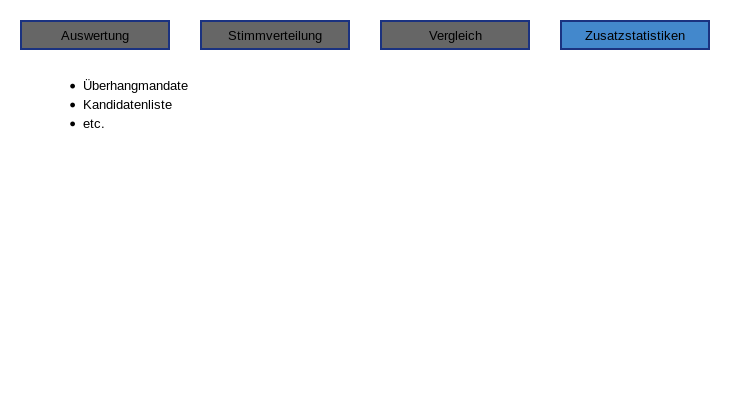
\includegraphics[width=\textwidth]{04-Zusatzstatistiken}}
    \end{center}
    \caption{Zusätzliche Statistiken, z.b. Liste von Überhangmandaten, etc.}
    \label{fig:gui-zusatzstatistiken}
\end{figure}
\subsection{Hinweise zur Zugangsberechtigung}
Für das Web-Frontend müssen keine Zugangsberechtigungen beachtet werden, da
dieses nur eine Auswertung der Daten zur Verfügung stellt, ein Schreibzugriff
auf die Daten jedoch nicht möglich sein soll.\\
Ein Zugriff auf die Datenbank sowie jegliche andere Möglichkeit, die
gespeicherten Daten zu ändern, darf nicht öffentlich zugänglich sein, sondern
bedarf einer Zugangsberechtigung.
\newpage
\section{Datenmodell}
\begin{figure}[h!]
    \begin{center}
        \fbox{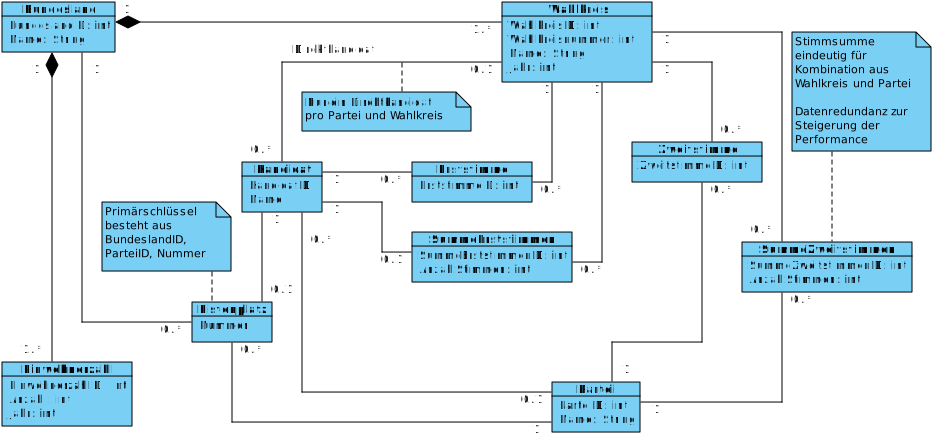
\includegraphics[width=\textwidth]{Datenmodell}}
    \end{center}
    \caption{Datenmodell}
    \label{fig:datenmodell}
\end{figure}
\section{Glossar}
\begin{itemize}
    \item API: Festgelegte Programmier-Schnittstelle, welche sich auch bei
        internen Änderungen an der Implementierung der Bibliothek nicht ändert.
    \item Batch-Loading: Einfügen von mehreren Stimmen auf ein Mal in die
        Datenbank, möglicherweise basierend auf aggregierten Daten
\end{itemize}
\end{document}
